\section{Exercises}

\begin{enumerate}[leftmargin=*]
%\item Determine whether the statement is {\bf True} or {\bf False}.
%\begin{enumerate}
%%\item If $N$ is an even integer then the vector $\bs{f}_{N/2}$ in the Fourier basis of $\mathbb{C}^N$ has real entries.
%%\item Let $\bs{x} \in \mathbb{R}^N$ and let $\bs{y} = \mathrm{DFT}(\bs{x})$. Then $\overline{\bs{x}[k]} = \bs{x}[N-k]$ for all $0<k<N$.
%\end{enumerate}
\item Suppose a signal $\bs{x}$ of length 9 has real values and let $\bs{y} = \mathrm{DFT}(\bs{x})$. Determine all the values of $\bs{y}$ given the values at even indices
$$
\bs{y}[0] = 1 \hspace{5mm}
\bs{y}[2] = 2+i \hspace{5mm}
\bs{y}[4] = 1+2i \hspace{5mm}
\bs{y}[6] = 1-3i \hspace{5mm}
\bs{y}[8] = 1-i
$$
\item Find a formula for $\bs{x}$ as a sum of sinusoids given
$$
\mathrm{DFT}(\bs{x}) = \begin{bmatrix} 1 & 3-3i & 2\sqrt{3}+2i& -4i& 4i &2\sqrt{3}-2i & 3+3i \end{bmatrix}^T
$$
\item Sketch the signal $\bs{x}$ such that the magnitude and phase plots of $\bs{y} = \mathrm{DFT}(\bs{x})$ are
\begin{center}
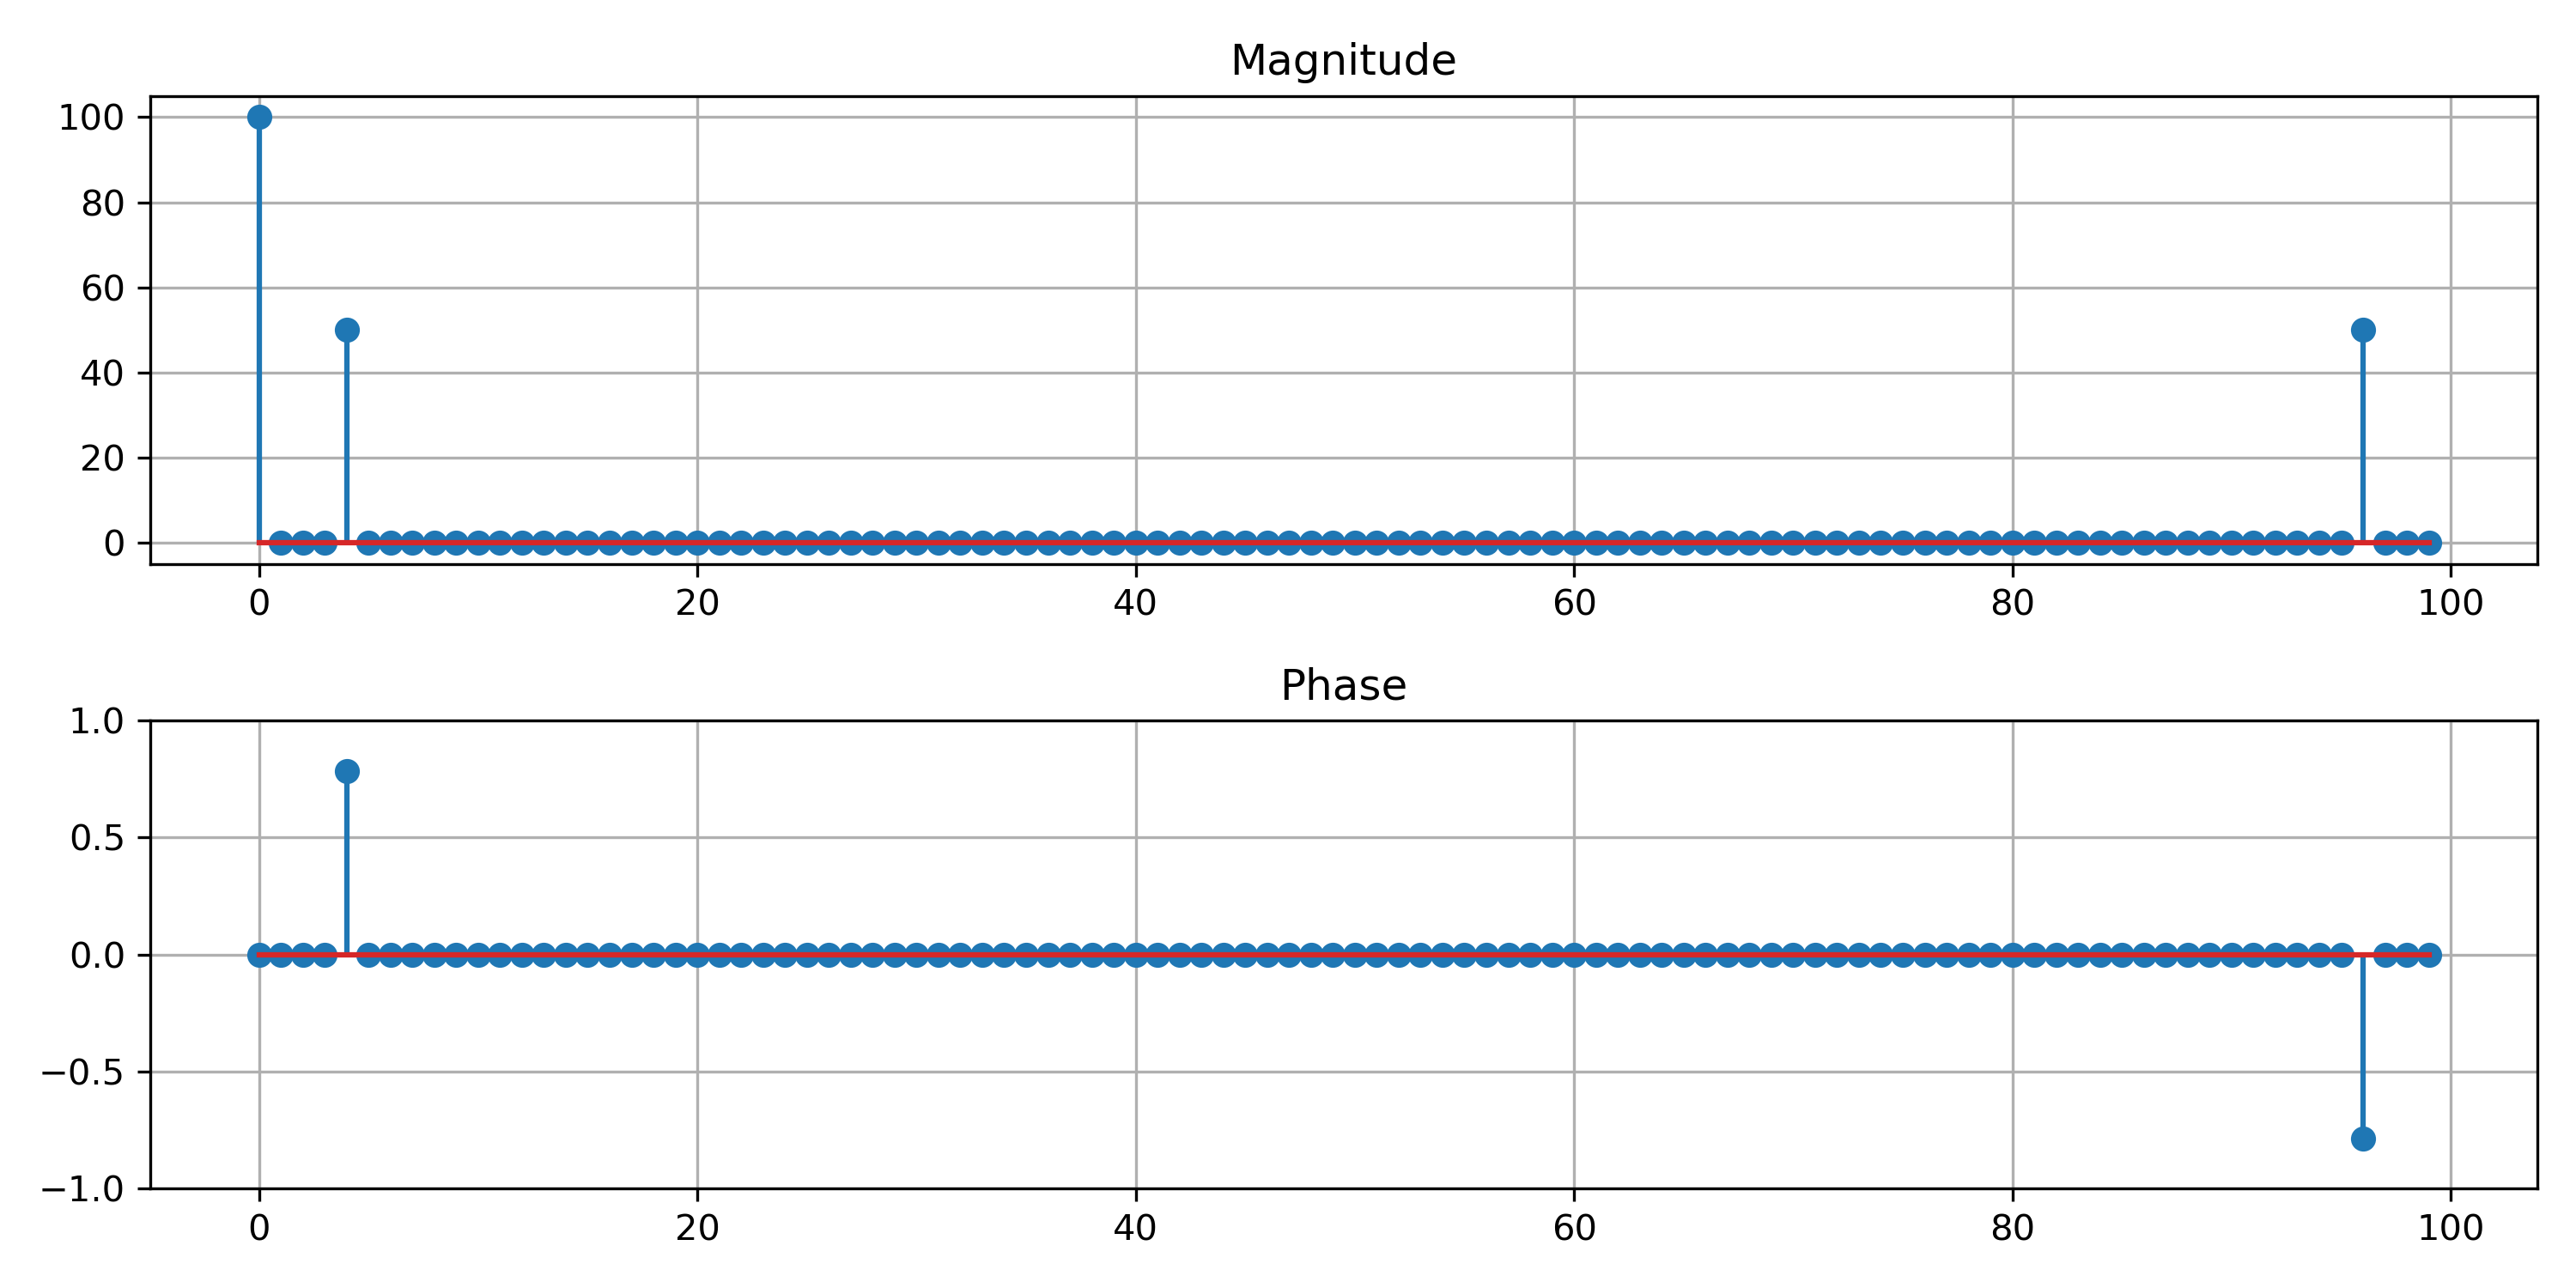
\includegraphics[width=4in]{04_ex02.png}
\end{center}
\item Let $\bs{x} = \begin{bmatrix} 1 & -1 & 2 & 1 \end{bmatrix}^T$. Compute $\mathrm{DFT}(\bs{x})$ using the fast Fourier transform. Compute $\mathrm{DFT}(\bs{x})$ also by $F_4$ and verify it is the same result.
\item Let $\bs{x} = \begin{bmatrix} 1 & 1 & 0 & 2 & 1 & 2 & 0 & -1 \end{bmatrix}^T$. Compute $\mathrm{DFT}(\bs{x})$ using the fast Fourier transform.
\item Let $N$ be an even integer and let $\bs{x} \in \mathbb{R}^N$ such that $\bs{x}[n] = 1$ if $n$ is even and $\bs{x}[n] = 0$ if $n$ is odd. Find $\mathrm{DFT}(\bs{x})$.
\item Let $N$ be an even integer and let $\bs{x} \in \mathbb{R}^N$ such that $\bs{x}[n] = 1$ if $n$ is even and $\bs{x}[n] = -1$ if $n$ is odd. Find $\mathrm{DFT}(\bs{x})$.
\item Let $N$ be an integer and let $\bs{x} \in \mathbb{R}^N$ such that $\bs{x}[0] = 0$ and $\bs{x}[n] = 1$ for $0<n<N$. Find $\mathrm{DFT}(\bs{x})$.
\item Run the following Python code for different values $N$:
\begin{verbatim}
N = 100
x = np.random.rand(N)
y = np.fft.fft(x)
plt.stem(np.abs(y),use_line_collection=True)
plt.show()
\end{verbatim}
Describe the magnitude plot and explain why it has the same general shape for each random sample. (Recall {\tt np.random.rand} samples from the uniform distribution on $[0,1]$.)
\newpage
\item Match the signal with the magnitude plot of its discrete Fourier transform.
\begin{center}
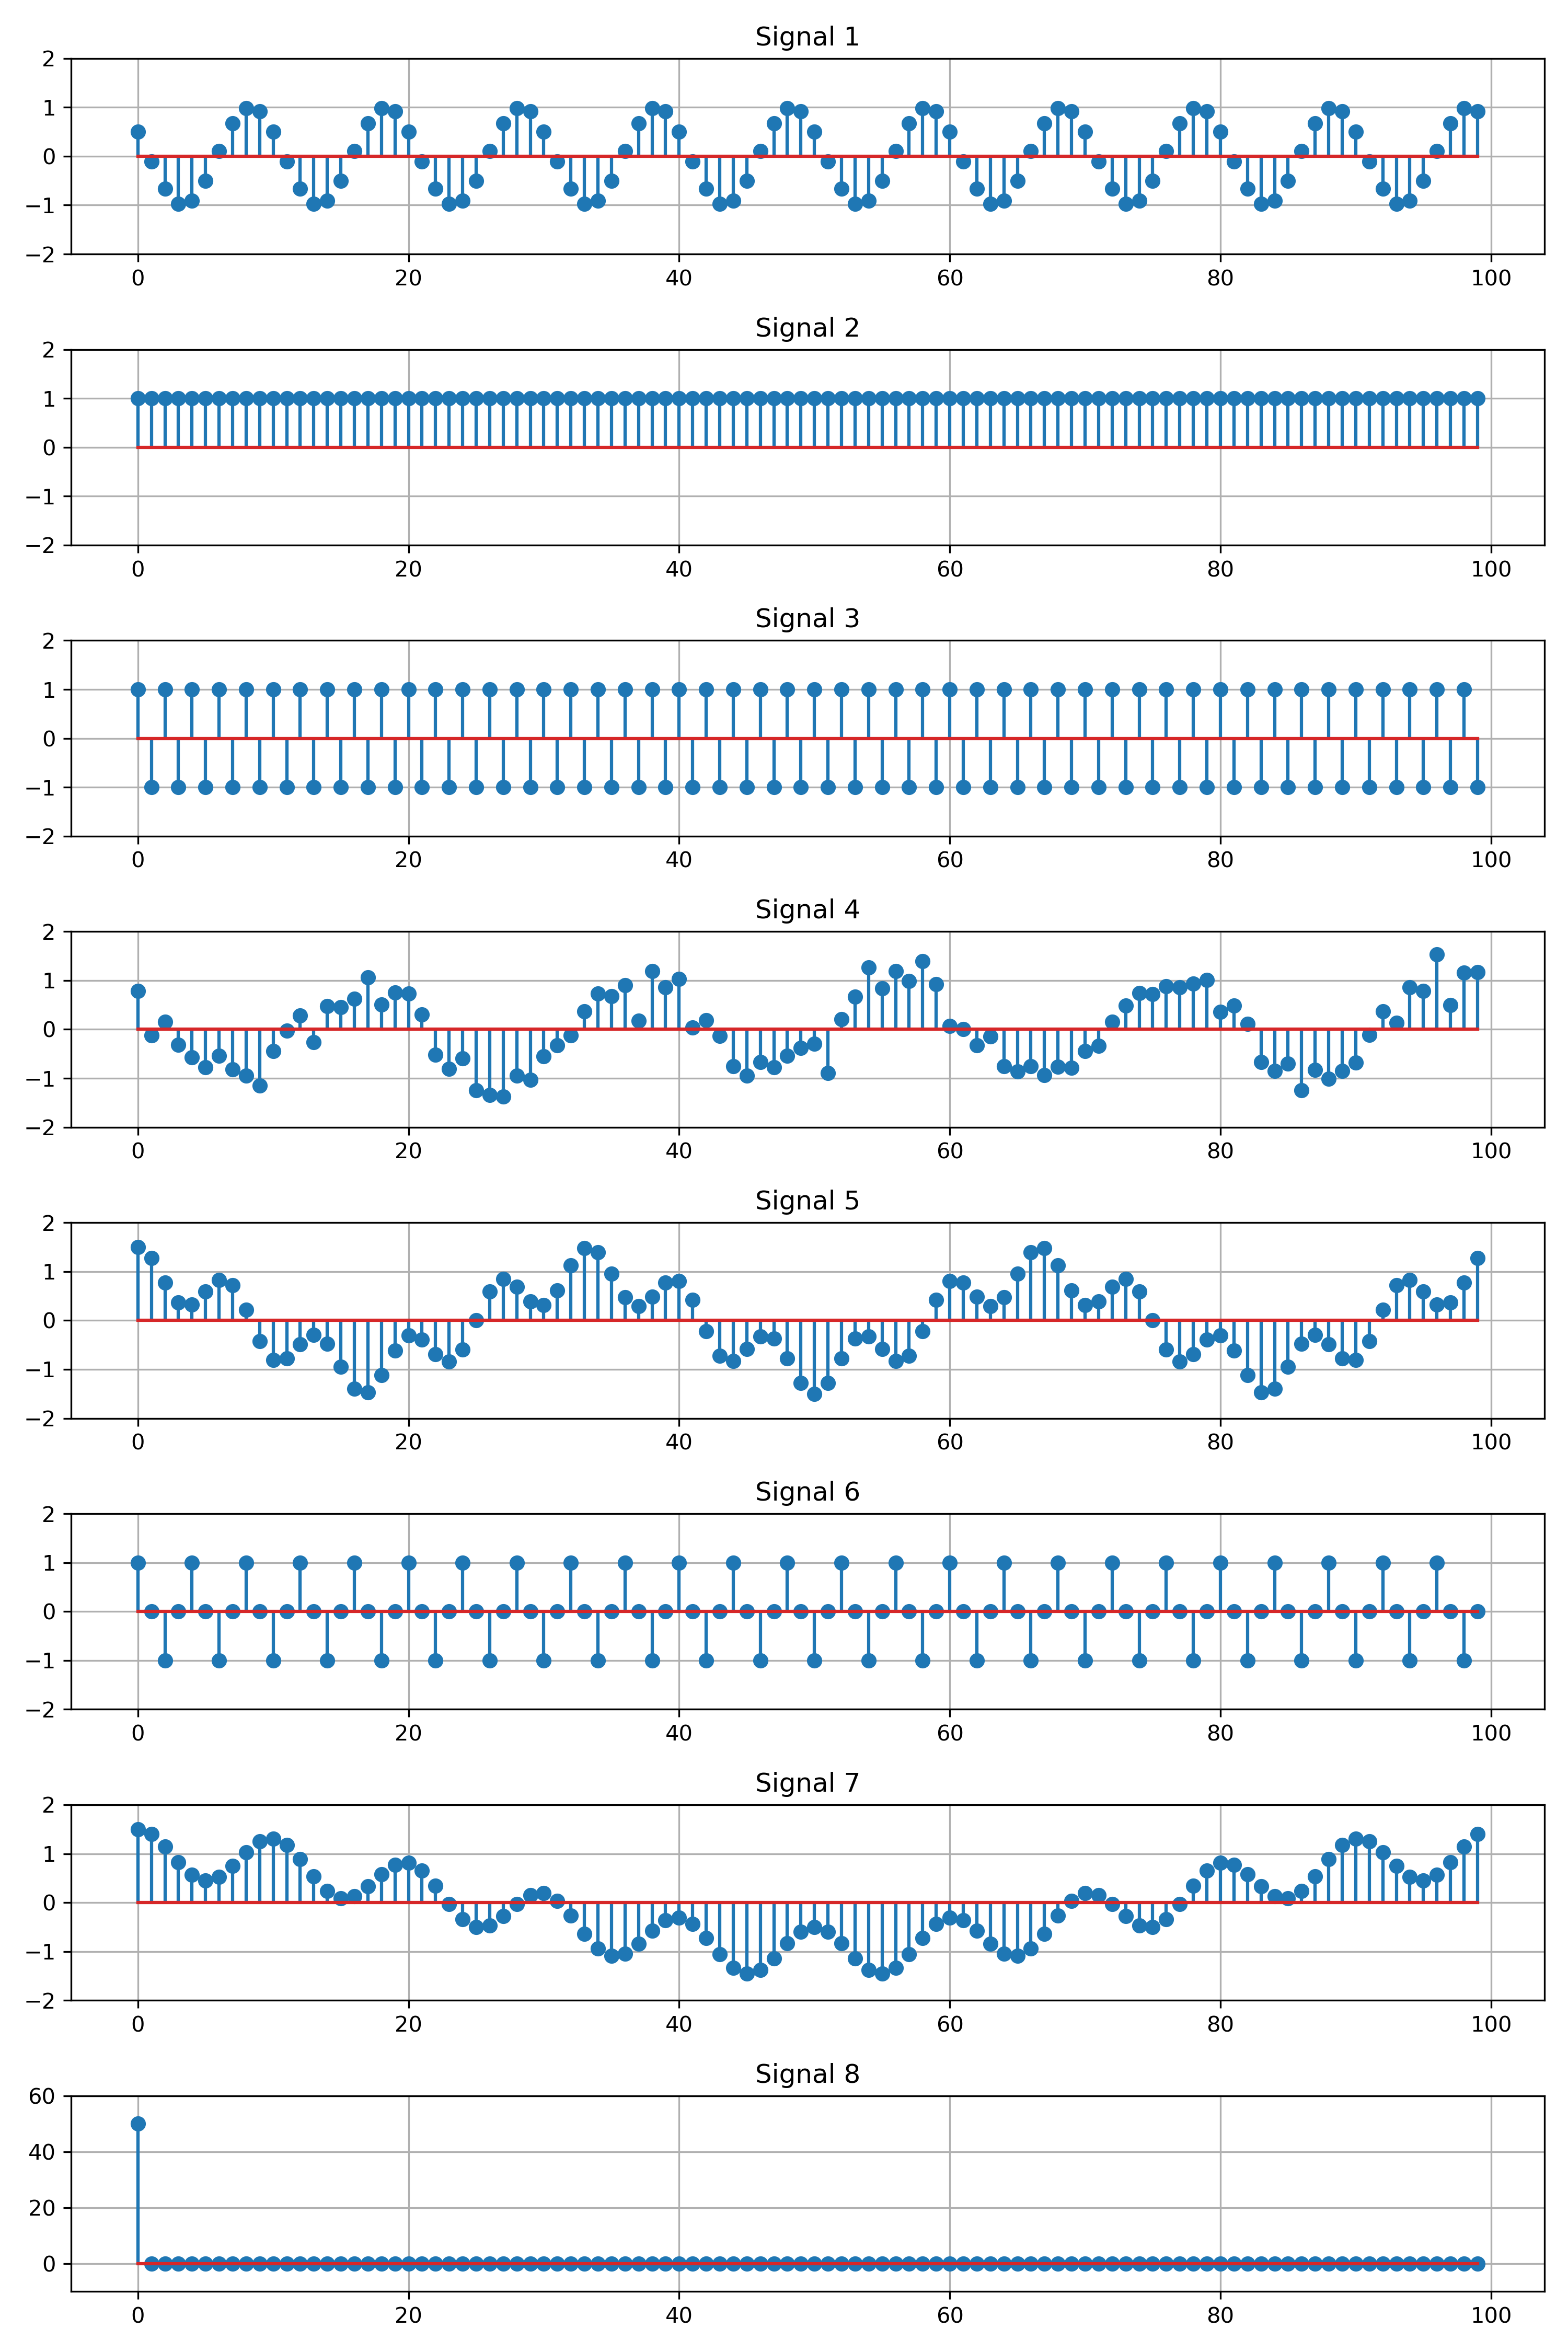
\includegraphics[height=8.5in]{04_ex01a.png}
\end{center}
\begin{center}
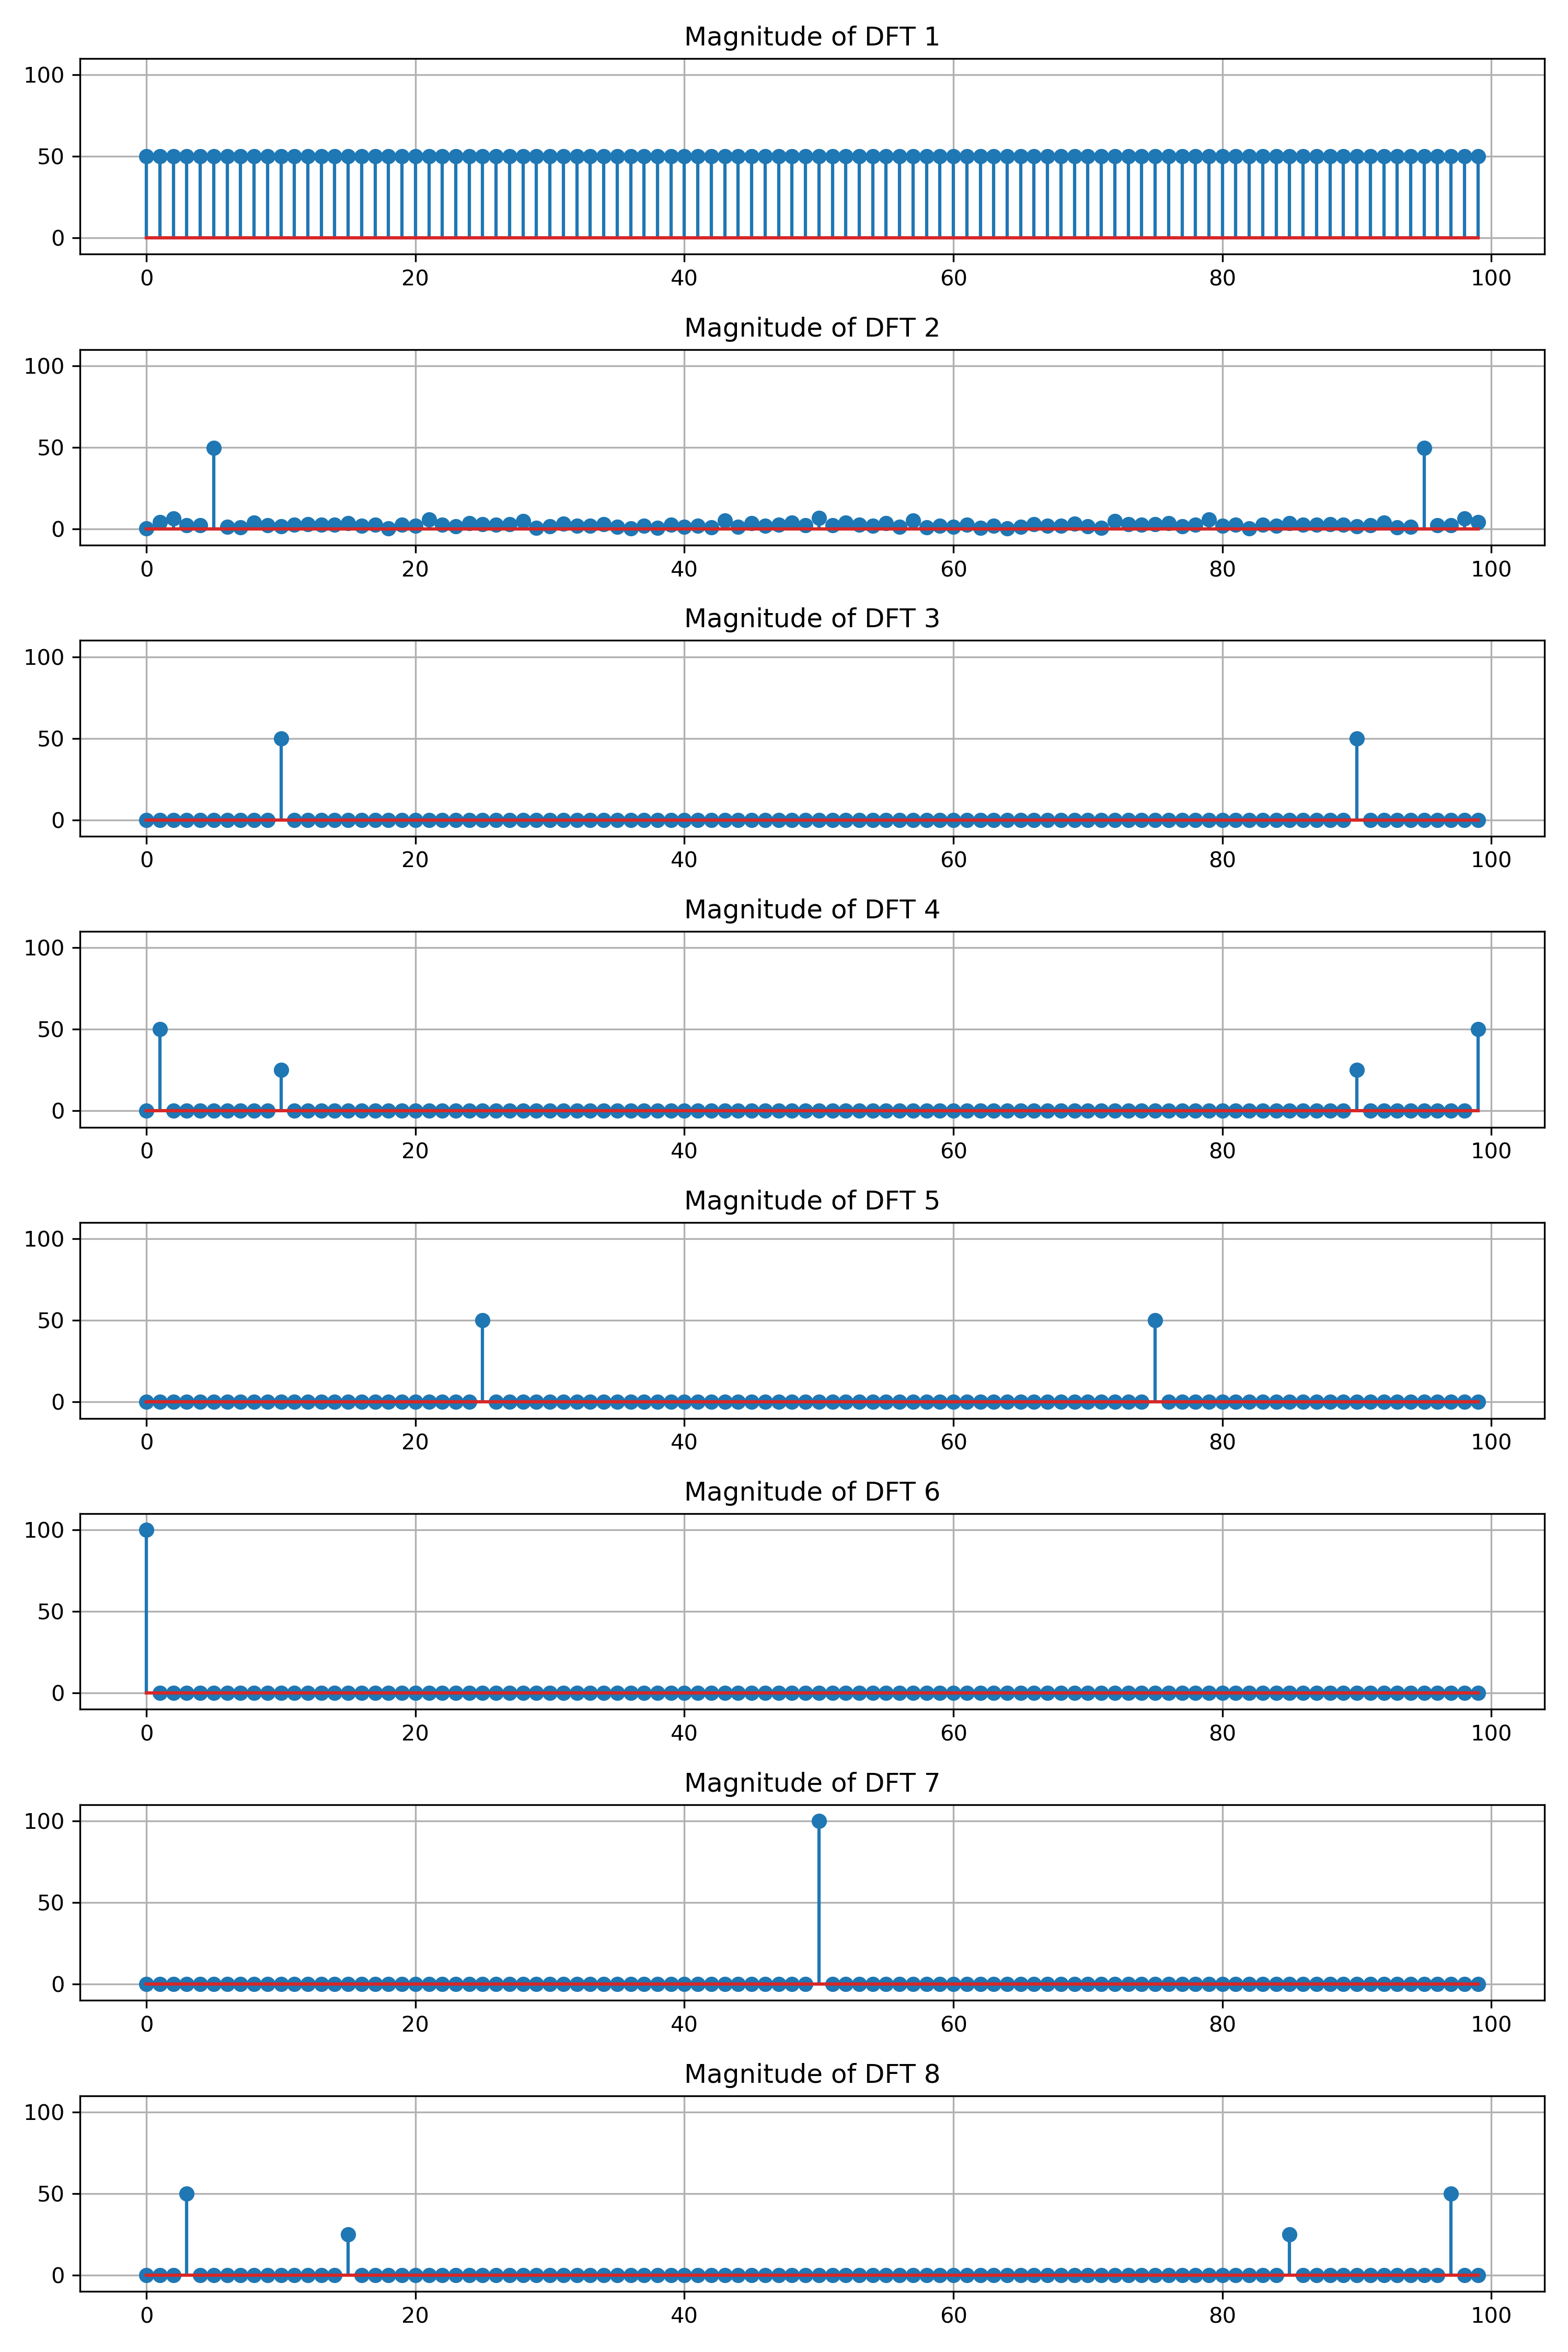
\includegraphics[height=8.75in]{04_ex01b.png}
\end{center}
\end{enumerate}